%File: anonymous-submission-latex-2024.tex
\documentclass[letterpaper]{article} % DO NOT CHANGE THIS
\usepackage[submission]{aaai24}  % DO NOT CHANGE THIS
\usepackage{times}  % DO NOT CHANGE THIS
\usepackage{helvet}  % DO NOT CHANGE THIS
\usepackage{courier}  % DO NOT CHANGE THIS
\usepackage[hyphens]{url}  % DO NOT CHANGE THIS
\usepackage{graphicx} % DO NOT CHANGE THIS
\urlstyle{rm} % DO NOT CHANGE THIS
\def\UrlFont{\rm}  % DO NOT CHANGE THIS
\usepackage{natbib}  % DO NOT CHANGE THIS AND DO NOT ADD ANY OPTIONS TO IT
\usepackage{caption} % DO NOT CHANGE THIS AND DO NOT ADD ANY OPTIONS TO IT
\frenchspacing  % DO NOT CHANGE THIS
\setlength{\pdfpagewidth}{8.5in} % DO NOT CHANGE THIS
\setlength{\pdfpageheight}{11in} % DO NOT CHANGE THIS
%
% These are recommended to typeset algorithms but not required. See the subsubsection on algorithms. Remove them if you don't have algorithms in your paper.
\usepackage{algorithm}
\usepackage{algorithmic}

% Custom packages
\usepackage{tikz}

%
% These are are recommended to typeset listings but not required. See the subsubsection on listing. Remove this block if you don't have listings in your paper.
\usepackage{newfloat}
\usepackage{listings}
\DeclareCaptionStyle{ruled}{labelfont=normalfont,labelsep=colon,strut=off} % DO NOT CHANGE THIS
\lstset{%
	basicstyle={\footnotesize\ttfamily},% footnotesize acceptable for monospace
	numbers=left,numberstyle=\footnotesize,xleftmargin=2em,% show line numbers, remove this entire line if you don't want the numbers.
	aboveskip=0pt,belowskip=0pt,%
	showstringspaces=false,tabsize=2,breaklines=true}
\floatstyle{ruled}
\newfloat{listing}{tb}{lst}{}
\floatname{listing}{Listing}
%
% Keep the \pdfinfo as shown here. There's no need
% for you to add the /Title and /Author tags.
\pdfinfo{
/TemplateVersion (2024.1)
}

% DISALLOWED PACKAGES
% \usepackage{authblk} -- This package is specifically forbidden
% \usepackage{balance} -- This package is specifically forbidden
% \usepackage{color (if used in text)
% \usepackage{CJK} -- This package is specifically forbidden
% \usepackage{float} -- This package is specifically forbidden
% \usepackage{flushend} -- This package is specifically forbidden
% \usepackage{fontenc} -- This package is specifically forbidden
% \usepackage{fullpage} -- This package is specifically forbidden
% \usepackage{geometry} -- This package is specifically forbidden
% \usepackage{grffile} -- This package is specifically forbidden
% \usepackage{hyperref} -- This package is specifically forbidden
% \usepackage{navigator} -- This package is specifically forbidden
% (or any other package that embeds links such as navigator or hyperref)
% \indentfirst} -- This package is specifically forbidden
% \layout} -- This package is specifically forbidden
% \multicol} -- This package is specifically forbidden
% \nameref} -- This package is specifically forbidden
% \usepackage{savetrees} -- This package is specifically forbidden
% \usepackage{setspace} -- This package is specifically forbidden
% \usepackage{stfloats} -- This package is specifically forbidden
% \usepackage{tabu} -- This package is specifically forbidden
% \usepackage{titlesec} -- This package is specifically forbidden
% \usepackage{tocbibind} -- This package is specifically forbidden
% \usepackage{ulem} -- This package is specifically forbidden
% \usepackage{wrapfig} -- This package is specifically forbidden
% DISALLOWED COMMANDS
% \nocopyright -- Your paper will not be published if you use this command
% \addtolength -- This command may not be used
% \balance -- This command may not be used
% \baselinestretch -- Your paper will not be published if you use this command
% \clearpage -- No page breaks of any kind may be used for the final version of your paper
% \columnsep -- This command may not be used
% \newpage -- No page breaks of any kind may be used for the final version of your paper
% \pagebreak -- No page breaks of any kind may be used for the final version of your paperr
% \pagestyle -- This command may not be used
% \tiny -- This is not an acceptable font size.
% \vspace{- -- No negative value may be used in proximity of a caption, figure, table, section, subsection, subsubsection, or reference
% \vskip{- -- No negative value may be used to alter spacing above or below a caption, figure, table, section, subsection, subsubsection, or reference

\setcounter{secnumdepth}{0} %May be changed to 1 or 2 if section numbers are desired.

% The file aaai24.sty is the style file for AAAI Press
% proceedings, working notes, and technical reports.
%

% Title

% Your title must be in mixed case, not sentence case.
% That means all verbs (including short verbs like be, is, using,and go),
% nouns, adverbs, adjectives should be capitalized, including both words in hyphenated terms, while
% articles, conjunctions, and prepositions are lower case unless they
% directly follow a colon or long dash
\title{FedKit---A Cross-Platform SDK for Mobile Federated Learning Research}
\author{
    %Authors
    % All authors must be in the same font size and format.
    Written by AAAI Press Staff\textsuperscript{\rm 1}\thanks{With help from the AAAI Publications Committee.}\\
    AAAI Style Contributions by Pater Patel Schneider,
    Sunil Issar,\\
    J. Scott Penberthy,
    George Ferguson,
    Hans Guesgen,
    Francisco Cruz\equalcontrib,
    Marc Pujol-Gonzalez\equalcontrib
}
\affiliations{
    %Afiliations
    \textsuperscript{\rm 1}Association for the Advancement of Artificial Intelligence\\
    % If you have multiple authors and multiple affiliations
    % use superscripts in text and roman font to identify them.
    % For example,

    % Sunil Issar\textsuperscript{\rm 2},
    % J. Scott Penberthy\textsuperscript{\rm 3},
    % George Ferguson\textsuperscript{\rm 4},
    % Hans Guesgen\textsuperscript{\rm 5}
    % Note that the comma should be placed after the superscript

    1900 Embarcadero Road, Suite 101\\
    Palo Alto, California 94303-3310 USA\\
    % email address must be in roman text type, not monospace or sans serif
    proceedings-questions@aaai.org
%
% See more examples next
}

%Example, Single Author, ->> remove \iffalse,\fi and place them surrounding AAAI title to use it
\iffalse
\title{My Publication Title --- Single Author}
\author {
    Author Name
}
\affiliations{
    Affiliation\\
    Affiliation Line 2\\
    name@example.com
}
\fi

\iffalse
%Example, Multiple Authors, ->> remove \iffalse,\fi and place them surrounding AAAI title to use it
\title{My Publication Title --- Multiple Authors}
\author {
    % Authors
    First Author Name\textsuperscript{\rm 1},
    Second Author Name\textsuperscript{\rm 2},
    Third Author Name\textsuperscript{\rm 1}
}
\affiliations {
    % Affiliations
    \textsuperscript{\rm 1}Affiliation 1\\
    \textsuperscript{\rm 2}Affiliation 2\\
    firstAuthor@affiliation1.com, secondAuthor@affilation2.com, thirdAuthor@affiliation1.com
}
\fi

\begin{document}

\maketitle

\begin{abstract}
    TODO
\end{abstract}

\section{Introduction}
The most appealing area of application for FL is mobile devices.
Yet, we could not find enough support for our real-world cross-platform mobile
FL research.
So, we purposefully built FedKit to power our mobile app for FL research.

PySyft \cite{ryffel2018generic,Ziller2021,hall2021syft}
does support cross-platform on-device training,
but its home-brew implementation is inefficient.

FedML \cite{he2020fedml} forces users to use a proprietary backend and
does not support iOS.

Most other FL frameworks do not support on-device training.

\section{System Description}

\newcommand{\model}{$M$}
\newcommand{\fs}{$S_F$}

FedKit powers a Federated Learning system that
consists of a single Backend Server and a set of mobile clients.
The clients communicate with the Backend to federate learning
using their local data,
by on-device training and exchanging ML models and parameters.

\subsection{Features}

\subsubsection{General Approachability}
FedKit allows ML researchers to develop ML models to target mobile devices
using Python libraries that they are already familiar with.
We integrate TensorFlow Lite to support Android training and Core ML for iOS
training,
both of which support converting models from popular libraries such as Pytorch,
TensorFlow, and Scikit-Learn.
% FIX: This is not that true about iOS.

\subsubsection{Backend-Oriented Model Deployment}
Researchers can deploy new models simply from the Backend,
without the need to update the mobile apps.
Most FL frameworks assume a fixed ML model that is bundled with the app,
making it difficult to iterate on the ML models.
By moving to our Backend the responsibility to choose which ML model to train,
we make it trivial to deploy new models that take the same kind of inputs and
outputs as the old one.

\subsubsection{Standardized On-Device Training}
On-device training is by far the most challenging part of FL because
the libraries involved are complex, experimental, poorly documented
and lack of community guidance.
FedKit simplifies this integration by providing implementation libraries
that wraps on-device training libraries and
only provides the functionality required by FL.

% TODO: Maybe merge checkpointing & telemetry.
\subsubsection{Full Model Checkpointing}
On every round of training an ML model \model,
all the parameters of \model{} is saved to the Backend database.
When \model{} is used for the next session of training,
its latest checkpoint is restored.

\subsubsection{Optional Telemetry}
On each round of training and evaluation,
we allow optional telemetry information to be sent to the Backend.
This includes the timing and loss,
associated with the FL session and the participants' ID.
This extra information helps FL researchers observe and analyze
the performance of their models.

\subsection{FL Workflow}

\begin{figure}
\centering
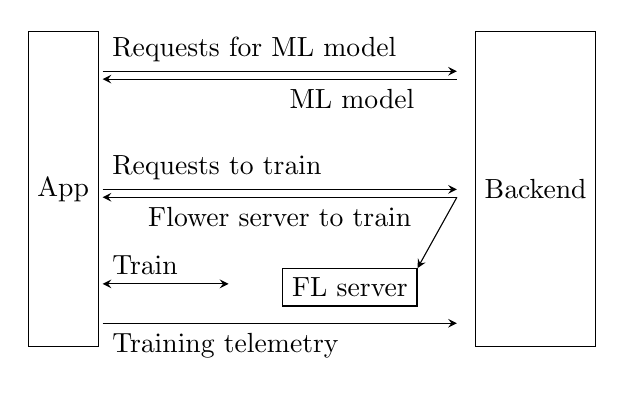
\begin{tikzpicture}
    \node[draw, minimum height=4cm] at (0, 0) {App};
    \node[draw, minimum height=4cm] at (6, 0) {Backend};
    \draw[-stealth] (0.5, 1.5) node[above right]{Requests for ML model} --
                    (5.0, 1.5);
    \draw[stealth-] (0.5, 1.4) -- node[below right]{ML model \model}
                    (5.0, 1.4);
    \draw[-stealth] (0.5, 0.0) node[above right]{Requests to train \model} --
                    (5.0, 0.0);
    \draw[stealth-] (0.5,-0.1) -- node[below]{Flower server to train \model}
                    (5.0,-0.1);
    \draw[stealth-] (4.5,-1.0) node[below left, draw]{FL server \fs} --
                    (5.0,-0.1);
    \draw[stealth-stealth] (0.5,-1.2) node[above right]{Train \model} --
                           (2.1,-1.2);
    \draw[-stealth] (0.5,-1.7) node[below right]{Training telemetry} --
                    (5.0,-1.7);
\end{tikzpicture}
\caption{FL workflow}
\label{fig:fl-workflow}
\end{figure}

Mobile clients fetch ML models from the Backend Server before doing FL.
This workflow allows Backend-oriented model deployment, where researches can
deploy new ML models simply by uploading them to the Backend,
without updating the client mobile apps.

\subsubsection{Data Type}
Each client has its Data Type, the shape of its training input and label,
predefined.
This makes sense because obtaining each client's training data requires
implementation specific to that client.

\subsubsection{Model Request}
Clients provide the Backend their Data Type and request for an ML model \model.

\subsubsection{Training Initiation}
Clients request the Backend to start training \model.
The Backend spawns an FL Server \fs{} and responds directs clients to it.

\subsubsection{Training}
Clients connect to \fs{} and participate in FL with their local data.
\fs{} schedules the training, aggregation and evaluation for \model;
it also sends aggregated parameters to the Backend for analysis.
Clients send telemetry about timing and loss to the Backend.

\subsection{Implementation}

We offer an example Flutter client implementation that supports both Android and
iOS, and a separate Kotlin Android client.

The clients make JSON APIs calls to the Backend,
and gRPC calls to FL Servers.
For that, we offer a Flutter package and a Kotlin package.

The Backend Server is designed as a persistent orchestrator service.

On-device training is especially difficult because mobile devices have limited
compute power.
To achieve optimal performance, our implementation adopts native
solutions---TensorFlow Lite on Android and Core ML on iOS.
We offer an Android package for on-device training and a Python package for
TensorFlow Lite model conversion from any Keras model.

We leverage Flower \cite{beutel2020flower} for FL Servers.

\section{Conclusion and Future Work}

% TODO: Conclusion.

We may adopt other iOS training libraries to avoid the restrictions of Core
ML---it only supports updating convolution and inner product layers.
One promising candidate is ONNX Runtime.

Security is not a priority in FedKit but it is easy to extend.
Differential Privacy can be added simply by adding noise before the data is
used for training.
Transport Layer Security can be enabled by
using HTTPS instead of HTTP for the Backend and
enabling SSL in the gRPC setting for the FL Servers.

\appendix

\section*{Acknowledgments}
TODO

\bigskip

\bibliography{main}

\end{document}
